\documentclass[landscape,a0paper,fontscale=0.265]{baposter}

\usepackage{calc}
%\usepackage{fourier}
\newcommand\Warning{%
 \makebox[1.4em][c]{%
 \makebox[0pt][c]{\raisebox{.1em}{\small!}}%
 \makebox[0pt][c]{\color{red}\Large$\bigtriangleup$}}
}
\usepackage{graphicx}
\usepackage{amsmath}
\usepackage{amssymb}
\usepackage{relsize}
\usepackage{multirow}
\usepackage{rotating}
\usepackage{bm}
\usepackage{url}
\usepackage{cancel}
\usepackage{array}

\usepackage{graphicx}
\usepackage{xargs}
\usepackage{multicol}

\usepackage{enumitem}
%\usepackage{times}
%\usepackage{helvet}
%\usepackage{bookman}
\usepackage{palatino}
\usepackage{subfiles}


\usepackage{ragged2e}
\usepackage{setspace}

\usepackage{anyfontsize}


\usepackage{dirtree}
\usepackage{wrapfig}



\usepackage[pages=some]{background}

\newcommand{\captionfont}{\footnotesize}



\graphicspath{{../images/}}

\usepackage{empheq}
\usepackage{dsfont}
\usepackage{enumitem}
\usepackage{stmaryrd}

%%%%%%%% added by mainak %%%%%%%%%%%
\usepackage{mathsymbols}
\usepackage[scaled]{helvet}
%\usepackage{nimbussans}
\usepackage[T1]{fontenc}
\usepackage{subfigure}
\usepackage{bbm}

% Import tikz packages for subfiles
\usepackage{tikz}
\usetikzlibrary{arrows, positioning, calc}
\usetikzlibrary{decorations.pathreplacing, patterns}

\usepackage[ruled]{algorithm2e}
% change font size of algorithm
\SetAlFnt{\small}
\SetAlCapFnt{\small}
\SetAlCapNameFnt{\small}
\setlength{\algomargin}{0em}
\SetAlCapHSkip{0em}
\usepackage{algorithmic}

% MM: from https://github.com/olivierverdier/python-latex-highlighting/blob/master/pythonhighlight.sty :
\usepackage{pythonhighlight}
\definecolor{linkcolor}{RGB}{82, 82, 183}
\definecolor{keywordcolour}{RGB}{207,34,46}
\definecolor{stringcolour}{RGB}{26,62,115}
\definecolor{literatecolour}{RGB}{20,90,179}
\definecolor{specmethodcolour}{RGB}{137,90,225}
\definecolor{backcolour}{rgb}{0.95,0.95,0.92}
\lstset{     % add some missing python keywords
    emph={[8]with, as},
    emphstyle={[8]\color{keywordcolour}\bfseries},
    emph={[9]Objective, Dataset, Solver, BaseObjective, BaseDataset, BaseSolver},
    emphstyle={[9]\color{literatecolour}\bfseries},
}
% \usepackage{inconsolata}    % nicer mono font

%%%%%%%%%%%%%%%%%%%%%%%%%%%%%%%%%%%%

% \newtheorem{thm}{Theorem}

%%%%%%%%%%%%%%%%%%%%%%%%%%%%%%%%%%%%%%%%%%%%%%%%%%%%%%%%%%%%%%%%%%%%%%%%%%%%%%%%
%%%% Some math symbols used in the text
%%%%%%%%%%%%%%%%%%%%%%%%%%%%%%%%%%%%%%%%%%%%%%%%%%%%%%%%%%%%%%%%%%%%%%%%%%%%%%%%

%%%%%%%%%%%%%%%%%%%%%%%%%%%%%%%%%%%%%%%%%%%%%%%%%%%%%%%%%%%%%%%%%%%%%%%%%%%%%%%%
% Multicol Settings
%%%%%%%%%%%%%%%%%%%%%%%%%%%%%%%%%%%%%%%%%%%%%%%%%%%%%%%%%%%%%%%%%%%%%%%%%%%%%%%%
\setlength{\columnsep}{1.5em}
\setlength{\columnseprule}{0mm}

%%%%%%%%%%%%%%%%%%%%%%%%%%%%%%%%%%%%%%%%%%%%%%%%%%%%%%%%%%%%%%%%%%%%%%%%%%%%%%%%
% Save space in lists. Use this after the opening of the list
%%%%%%%%%%%%%%%%%%%%%%%%%%%%%%%%%%%%%%%%%%%%%%%%%%%%%%%%%%%%%%%%%%%%%%%%%%%%%%%%
\newcommand{\compresslist}{%
\setlength{\itemsep}{1pt}%
\setlength{\parskip}{0pt}%
\setlength{\parsep}{0pt}%
}

\def\myitem{{\color{linkcolor} $\blacktriangleright$}}
\renewcommand{\labelitemi}{\myitem}

%%%%%%%%%%%%%%%%%%%%%%%%%%%%%%%%%%%%%%%%%%%%%%%%%%%%%%%%%%%%%%%%%%%%%%%%%%%%%%
%%% Begin of Document
%%%%%%%%%%%%%%%%%%%%%%%%%%%%%%%%%%%%%%%%%%%%%%%%%%%%%%%%%%%%%%%%%%%%%%%%%%%%%%


\begin{document}

%%%%%%%%%%%%%%%%%%%%%%%%%%%%%%%%%%%%%%%%%%%%%%%%%%%%%%%%%%%%%%%%%%%%%%%%%%%%%%
%%% Here starts the poster
%%%---------------------------------------------------------------------------
%%% Format it to your taste with the options
%%%%%%%%%%%%%%%%%%%%%%%%%%%%%%%%%%%%%%%%%%%%%%%%%%%%%%%%%%%%%%%%%%%%%%%%%%%%%%
% Define some colors

%\definecolor{lightblue}{cmyk}{0.83,0.24,0,0.12}
\definecolor{lightblue}{rgb}{0.145,0.6666,1}
\definecolor{tpt}{RGB}{200,34,84}
\definecolor{goldengatered}{RGB}{255,41,46}
% \definecolor{orange}{RGB}{31,58,224}
%\definecolor{inriared}{HTML}{E52D37}

\def\maincolor{lightblue}

\newcommand{\mydot}{\hspace*{-0.3ex}%
\raisebox{0.2ex}{\color{\maincolor}\rule{1.1ex}{1.1ex}}%
\hspace*{0.4ex}%
}

\hyphenation{resolution occlusions}
%%
\begin{poster}%
  % Poster Options
  {
  % Show grid to help with alignment
  grid=false,
  columns=6,
  % Column spacing
  colspacing=0.35em,
  % Color style
  bgColorOne=white,
  bgColorTwo=lightblue,
  % borderColor=goldengatered,
  borderColor=black,
  % headerColorOne=goldengatered,
  headerColorOne=\maincolor,
  headerColorTwo=purple,
  headerFontColor=white,
  boxColorOne=white,
  boxColorTwo=lightblue,
  % Format of textbox
  textborder=rectangle,
  % Format of text header
  eyecatcher=true,
  headerborder=closed,
  % headerheight=0.148\textheight,
  headerheight=0.\textheight,
%  textfont=\sc, An example of changing the text font
  headershape=rectangle,
  headershade=plain,
  headerfont=\Large\fontfamily{\sfdefault}\bfseries, %Sans Serif
  textfont={\setlength{\parindent}{1.5em}},
  boxshade=plain,
 % background=shadelr,
  background=plain,
  linewidth=0.5pt
  }
  % Eye Catcher
  {
  % \rotatebox[origin=c]{-90}{\includegraphics[height=16em]{images/logo_inria.pdf}}
  % \begin{minipage}{.17\linewidth}
  %   \centering
  %   \includegraphics[width=0.6\linewidth]{example-image-a}
  % \end{minipage}
  }
  % Title
  {
    % \huge\fontfamily{\sfdefault}\bfseries {
    %   Learning step sizes for unfolded sparse coding
    % }
    % \vspace{.7em}
  }
  % Authors
  {
  %   \Large  {\textbf
  %   {
  %     Pierre Ablin$^{*}$, \hspace{5pt}
  %     Thomas Moreau$^{*}$, \hspace{5pt}
  %     Mathurin Massias, \hspace{5pt}
  %     Alexandre Gramfort}}\\
  %      \vspace{5pt}
  %  \normalsize{
  %  Univ. Paris-Saclay, INRIA, Parietal team, Saclay, France.
  %  $^*$ Contributed Equally
  %  \\}
  %  \vspace{-10pt}
  }
  % University logo
  {% The makebox allows the title to flow into the logo, this is a hack because of the L shaped logo.
    %\includegraphics[height=7.5em]{images/logo_sb.pdf}
    %\includegraphics[height=3.0em]{images/bilgi.jpg}
    % \begin{minipage}{.18\linewidth}
    %  \hfill
    %   \begin{minipage}{\linewidth}
    %     \centering
    %     \includegraphics[width=0.9\linewidth]{example-image-golden}\\
    %     \includegraphics[width=.8\linewidth]{example-image-golden}\\
    %   \end{minipage}
    % \end{minipage}
  }

%%%%%%%%%%%%%%%%%%%%%%%%%%%%%%%%%%%%%%%%%%%%%%%%%%%%%%%%%%%%%%%%%%%%%%%%%%%%%%
%%% Now define the boxes that make up the poster
%%%---------------------------------------------------------------------------
%%% Each box has a name and can be placed absolutely or relatively.
%%% The only inconvenience is that you can only specify a relative position
%%% towards an already declared box. So if you have a box attached to the
%%% bottom, one to the top and a third one which should be in between, you
%%% have to specify the top and bottom boxes before you specify the middle
%%% box.
%%%%%%%%%%%%%%%%%%%%%%%%%%%%%%%%%%%%%%%%%%%%%%%%%%%%%%%%%%%%%%%%%%%%%%%%%%%%%%

% A coloured circle useful as a bullet with an adjustably strong filling
\newcommand{\colouredcircle}{%
  \tikz{\useasboundingbox (-0.2em,-0.32em) rectangle(0.2em,0.32em);
        \draw[draw=black,fill=purple,line width=0.03em] (0,0) circle(0.18em);}
}


%%%%%%%%%%%%%%%%%%%%%%%%%%%%%%%%%%%%%%%%%%%%%%%%%%%%%%%%%%%%%%%%%%%%%%%%%%%%%%
\headerbox{Benchopt API}{name=api,column=0,row=0, span=4}{
%%%%%%%%%%%%%%%%%%%%%%%%%%%%%%%%%%%%%%%%%%%%%%%%%%%%%%%%%%%%%%%%%%%%%%%%%%%%%%
%
%%%%%%%%%%%%%%%%%%%%%%%%%%%%%%%%%%%
% Directory structure
%%%%%%%%%%%%%%%%%%%%%%%%%%%%%%%%%%%
\fcolorbox{black}{black!15}{
  \begin{minipage}{.20\textwidth}
    \vskip.3em
\dirtree{%
.1 benchmark/.
.2 objective.py.
.2 datasets/.
.3 dataset1.py.
.3 dataset2.py.
.2 solvers/.
.3 solver1.py.
.3 solver2.py.
}
\phantom{.}
\end{minipage}
}
%
%
\hskip4ex
%
%
%%%%%%%%%%%%%%%%%%%%%%%%%%%%%%%%%%%
% Schema API
%%%%%%%%%%%%%%%%%%%%%%%%%%%%%%%%%%%
\begin{minipage}{.7\textwidth}
  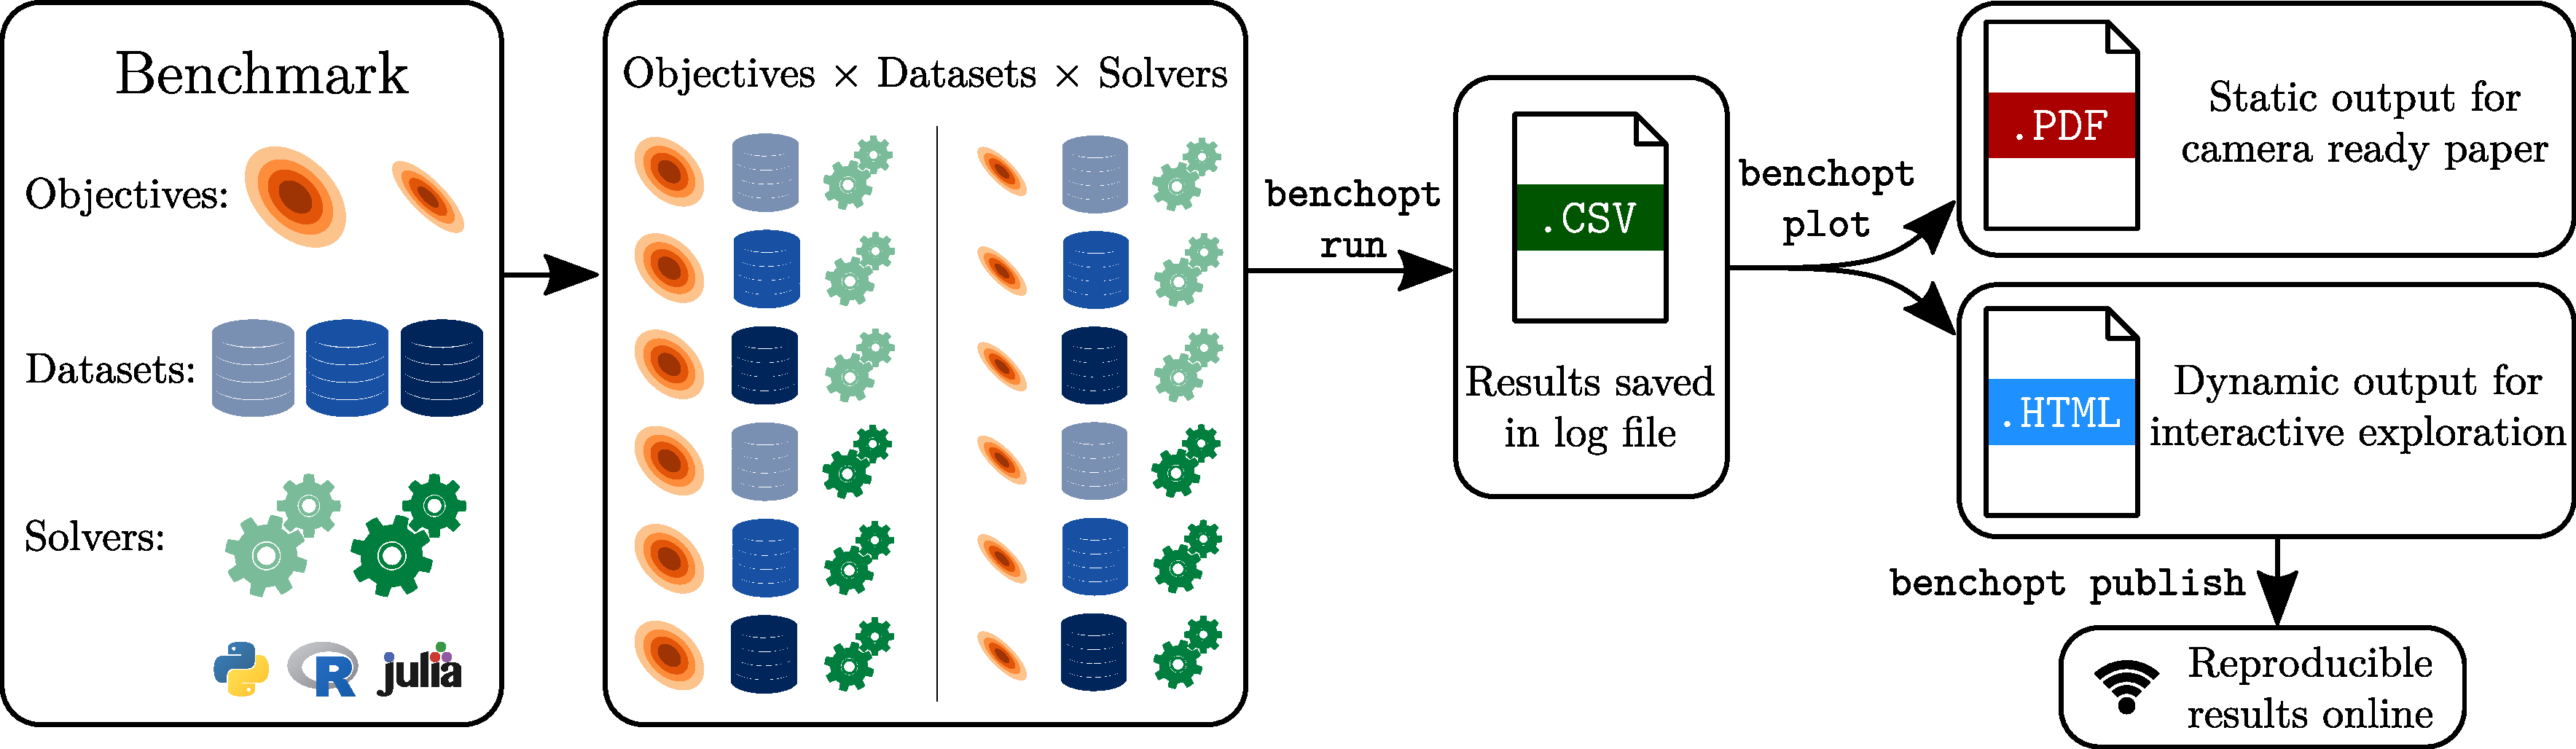
\includegraphics[width=\textwidth]{benchopt_schema_objectives_with_logos}
\end{minipage}

}

%%%%%%%%%%%%%%%%%%%%%%%%%%%%%%%%%%%%%%%%%%%%%%%%%%%%%%%%%%%%%%%%%%%%%%%%%%%%%
% Central eye-catching box
%%%%%%%%%%%%%%%%%%%%%%%%%%%%%%%%%%%%%%%%%%%%%%%%%%%%%%%%%%%%%%%%%%%%%%%%%%%%%
\begin{posterbox}[name=center,column=0,below=api,span=4,
  boxheaderheight=0em,
  boxColorOne=\maincolor,
  ]{}
%%%%%%%%%%%%%%%%%%%%%%%%%%%%%%%%%%%%%%%%%%%%%%%%%%%%%%%%%%%%%%%%%%%%%%%%%%%%%%



%
%%%%%%%%%%%%%%%%%%%%%%%
% Left box - goodies
%%%%%%%%%%%%%%%%%%%%%%%
\fcolorbox{black}{white}{
\begin{minipage}[c][16em]{.239\linewidth}
\raggedright
{\bf Research paper benchmarks:}
\begin{itemize}
\item Not transparent
\item Hard to reproduce
\item Time consuming
\item Frozen in time
\end{itemize}
\vskip1em\centering
{\bf Benchopt solves this!}\\
% {\bf Easy benchmark run:}
% \begin{itemize}
%   \item Modular and collaborative
%   \item Automatic caching
%   \item Parallelization with \texttt{joblib} and {SLURM}
%   \item Cross languages: R, Julia
% \end{itemize}
\end{minipage}
}
\hskip2ex
%
%%%%%%%%%%%%%%%%%%%%%%%
% Center Logo and QR code
%%%%%%%%%%%%%%%%%%%%%%%
\begin{minipage}{.39\linewidth}
\centering

\includegraphics[width=0.5\linewidth]{logo_benchopt}\\
{\color{white}\bf\Large Reproducible, Extendable and Shareable Benchmarks\\[.5em]}
\hfill

\includegraphics[width=0.2\linewidth]{qr-doc}\hfill

\includegraphics[width=0.2\linewidth]{qr-pdf}\hfill\phantom{.}\\
\raisebox{-.5em}{
\includegraphics[height=2em]{logo_github}} {\bf\color{white}~~https://github.com/benchopt/benchopt}
\end{minipage}
\hskip2ex
%
%%%%%%%%%%%%%%%%%%%%%%%%%%%%%%%%%%%%%
% Right box - publish information
%%%%%%%%%%%%%%%%%%%%%%%%%%%%%%%%%%%%
\fcolorbox{black}{white}{
\begin{minipage}[c][16em]{.239\linewidth}
\raggedright
{\bf Publishable results:}\\[.5em]
\centering
% 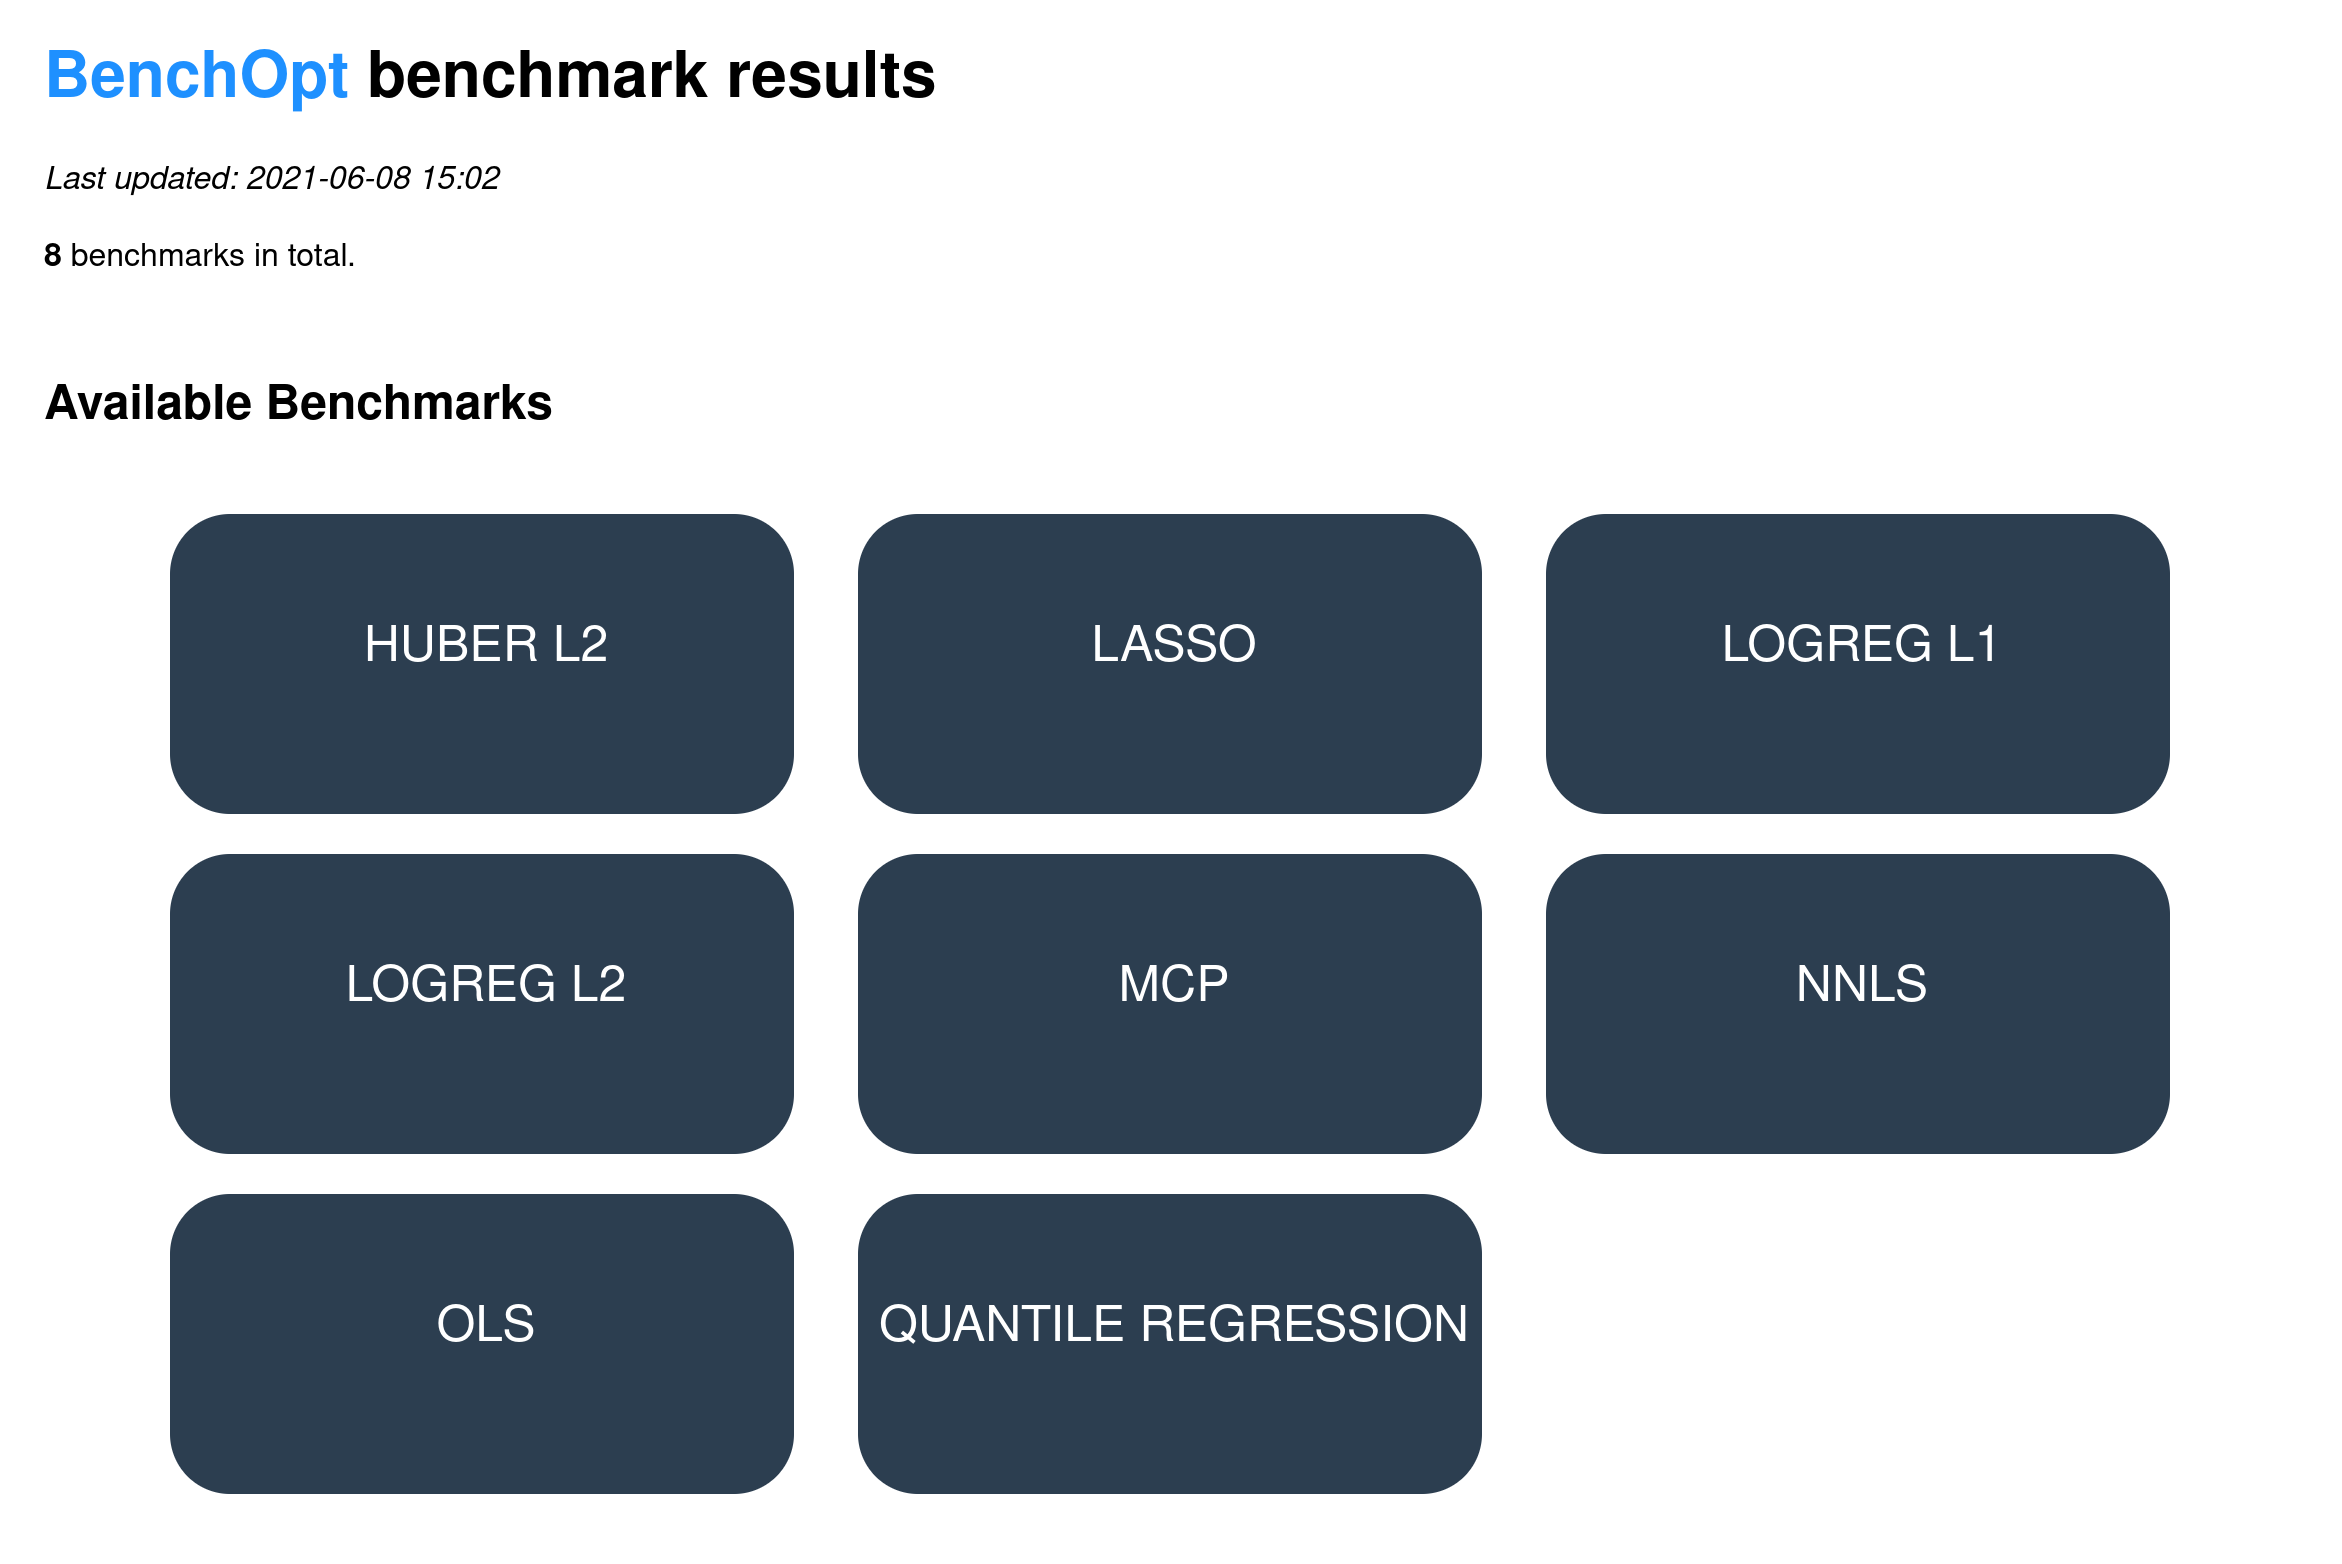
\includegraphics[width=0.45\linewidth]{benchopt_results}
\raisebox{-2ex}{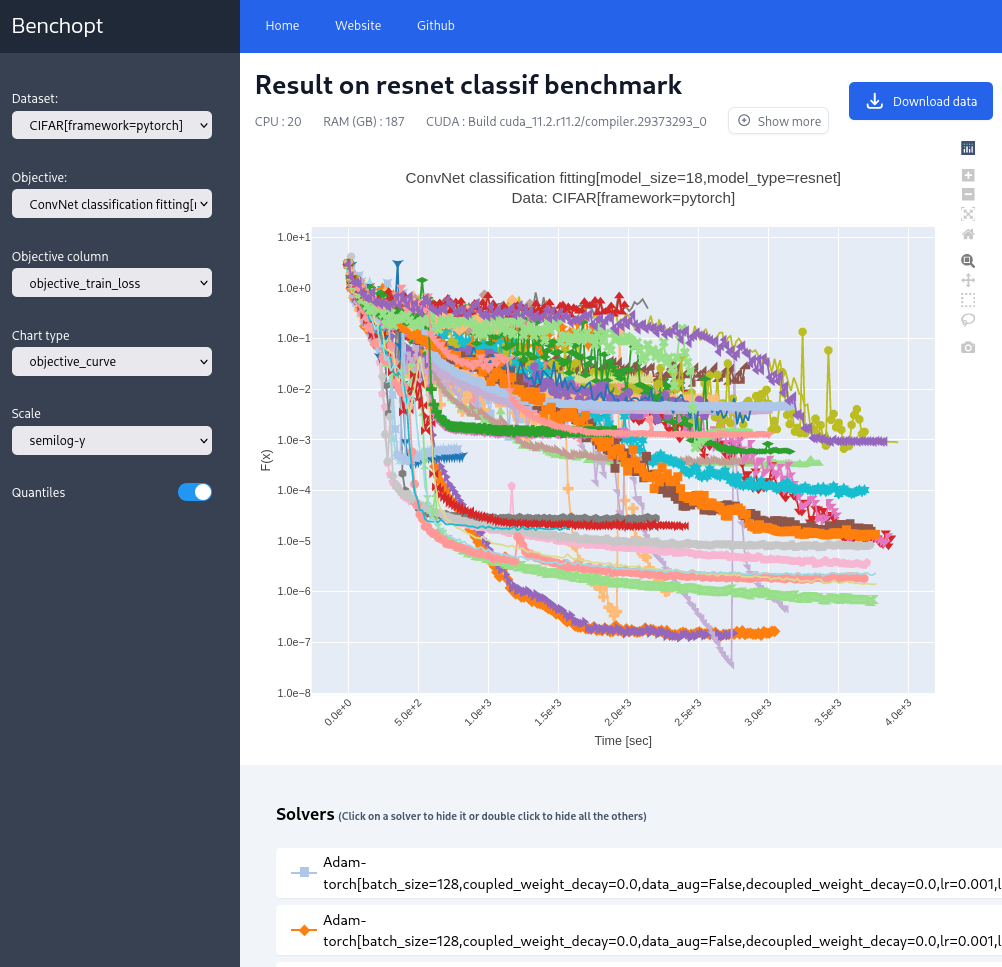
\includegraphics[width=0.95\linewidth]{benchopt_convnet}}
\end{minipage}
}
\end{posterbox}




%%%%%%%%%%%%%%%%%%%%%%%%%%%%%%%%%%%%%%%%%%%%%%%%%%%%%%%%%%%%%%%%%%%%%%%%%%%
% Example of Dataset
%%%%%%%%%%%%%%%%%%%%%%%%%%%%%%%%%%%%%%%%%%%%%%%%%%%%%%%%%%%%%%%%%%%%%%%%%%%
\begin{posterbox}[name=use-case-data,column=4,span=2, %below=center,
  boxColorOne=black!15,]{Adding a Dataset}
%%%%%%%%%%%%%%%%%%%%%%%%%%%%%%%%%%%%%%%%%%%%%%%%%%%%%%%%%%%%%%%%%%%%%%%%%%%

  \begin{python}
class Dataset(BaseDataset):
    name = "Simulated"

    parameters = {"n": [10, 100], "p": [10, 100]}

    def get_data(self):
        rng = np.random.RandomState(27)
        X = rng.randn(self.n, self.p)
        y = X @ rng.randn(self.p)
        return dict(X=self.X, y=self.y)

    \end{python}
    \vskip-1.8em\phantom{.}
\end{posterbox}


%%%%%%%%%%%%%%%%%%%%%%%%%%%%%%%%%%%%%%%%%%%%%%%%%%%%%%%%%%%%%%%%%%%%%%%%%%%
% Example of Objective
%%%%%%%%%%%%%%%%%%%%%%%%%%%%%%%%%%%%%%%%%%%%%%%%%%%%%%%%%%%%%%%%%%%%%%%%%%%
\begin{posterbox}[name=use-case-obj,column=4,span=2, below=use-case-data,
  boxColorOne=black!15]{Adding an Objective}
%%%%%%%%%%%%%%%%%%%%%%%%%%%%%%%%%%%%%%%%%%%%%%%%%%%%%%%%%%%%%%%%%%%%%%%%%%%

\begin{python}
class Objective(BaseObjective):
    name = "Least Square"

    def set_data(self, X, y):
        self.X, self.y = X, y

    def get_objective(self):
        return dict(X=self.X, y=self.y)

    def compute(self, w):
        res = self.y - self.X @ w
        return dict(value=.5 * res @ res, norm=w @ w)

\end{python}
\vskip-1.8em\phantom{.}
\end{posterbox}


%%%%%%%%%%%%%%%%%%%%%%%%%%%%%%%%%%%%%%%%%%%%%%%%%%%%%%%%%%%%%%%%%%%%%%%%%%%
% Example of Solver
%%%%%%%%%%%%%%%%%%%%%%%%%%%%%%%%%%%%%%%%%%%%%%%%%%%%%%%%%%%%%%%%%%%%%%%%%%%
\begin{posterbox}[name=use-case-solver,column=4,span=2, below=use-case-obj,
  boxColorOne=black!15,]{Adding a Solver}
%%%%%%%%%%%%%%%%%%%%%%%%%%%%%%%%%%%%%%%%%%%%%%%%%%%%%%%%%%%%%%%%%%%%%%%%%%%

\begin{python}
class Solver(BaseSolver):
    name = "GD"
    parameters = {"lr": [.1, .01]}

    def set_objective(self, X, y):
        self.X, self.y = X, y

    def run(self, n_iter):
        w = np.zeros(X.shape[1])
        for _ in range(n_iter):
            grad = X.T @ (X @ w - y)
            w -= self.lr * grad
            self.w_ = w

    def get_result(self):
        return self.w_
    \end{python}
    \vskip-1.8em\phantom{.}
\end{posterbox}



%%%%%%%%%%%%%%%%%%%%%%%%%%%%%%%%%%%%%%%%%%%%%%%%%%%%%%%%%%%%%%%%%%%%%%%%%%%%%%
% Benchmark resnet
%%%%%%%%%%%%%%%%%%%%%%%%%%%%%%%%%%%%%%%%%%%%%%%%%%%%%%%%%%%%%%%%%%%%%%%%%%%%%%
\headerbox{ResNet for Image Classification}{name=resnet,column=0,below=center,span=4,
bottomaligned=use-case-solver}{
%%%%%%%%%%%%%%%%%%%%%%%%%%%%%%%%%%%%%%%%%%%%%%%%%%%%%%%%%%%%%%%%%%%%%%%%%%%%%%
% \hskip-4ex
\begin{minipage}{.42\textwidth}
  \begin{itemize}\setlist{leftmargin=5.5mm}
    \item Image classification with ResNet18
    \item Evaluate the test loss
    \item Various optimization strategies:\\\emph{Data Aug., Weight Decay, Momentum, \dots}
    \item Compare \texttt{Pytorch} and \texttt{Tensorflow}
    \item Reproducible SOTA results for baselines
  \end{itemize}
\end{minipage}\hskip2ex
\begin{minipage}{.5\textwidth}
  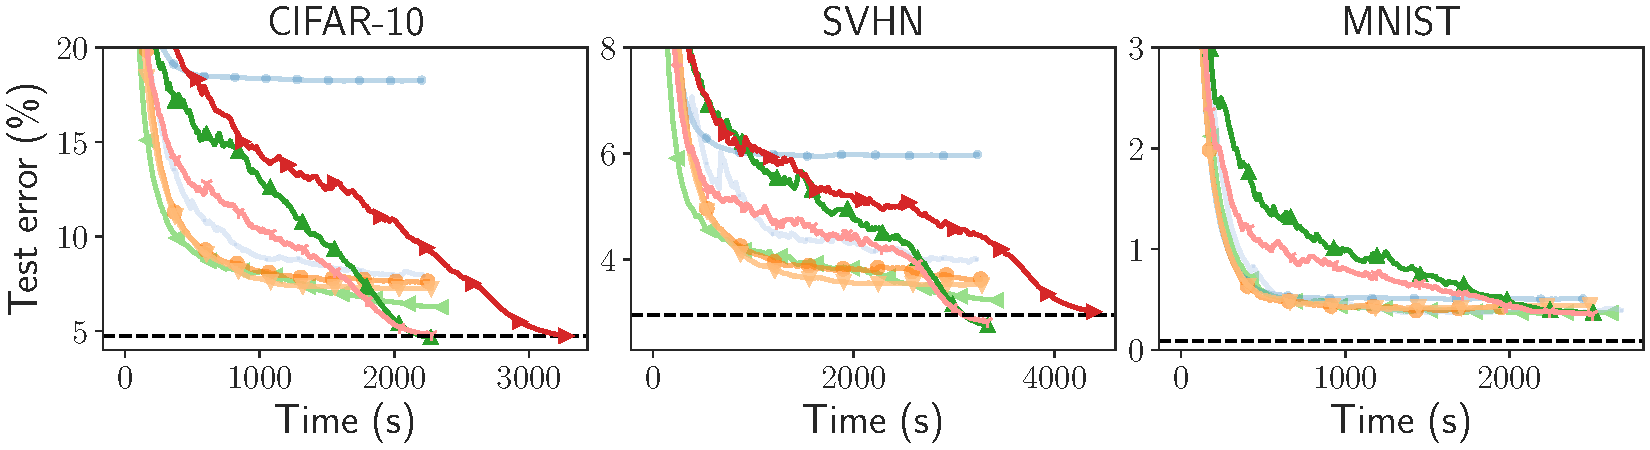
\includegraphics[width=\textwidth]{resnet18_sgd_torch}
  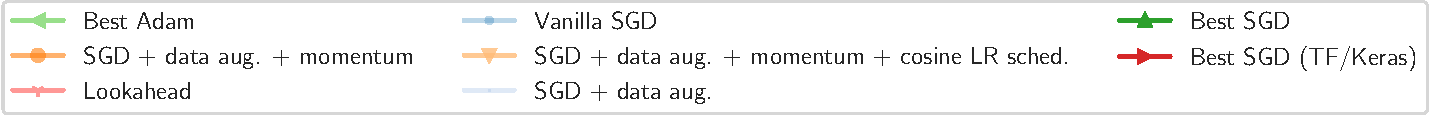
\includegraphics[width=\textwidth]{resnet18_sgd_torch_legend}
\end{minipage}%


}

% %%%%%%%%%%%%%%%%%%%%%%%%%%%%%%%%%%%%%%%%%%%%%%%%%%%%%%%%%%%%%%%%%%%%%%%%%%%%%%
% % Benchmark logreg
% %%%%%%%%%%%%%%%%%%%%%%%%%%%%%%%%%%%%%%%%%%%%%%%%%%%%%%%%%%%%%%%%%%%%%%%%%%%%%%
% \headerbox{$\ell_2$-regularized Logistic Regression}{name=logreg,column=3,below=resnet,span=3,bottomaligned=lasso}{
% %%%%%%%%%%%%%%%%%%%%%%%%%%%%%%%%%%%%%%%%%%%%%%%%%%%%%%%%%%%%%%%%%%%%%%%%%%%%%%

% \[
%   \min_\beta \sum_i \log(1 + \exp(-y_i x_i^\top \beta)) + \frac{\lambda}{2} \|\beta\|_2^2
% \]
% \centering
% 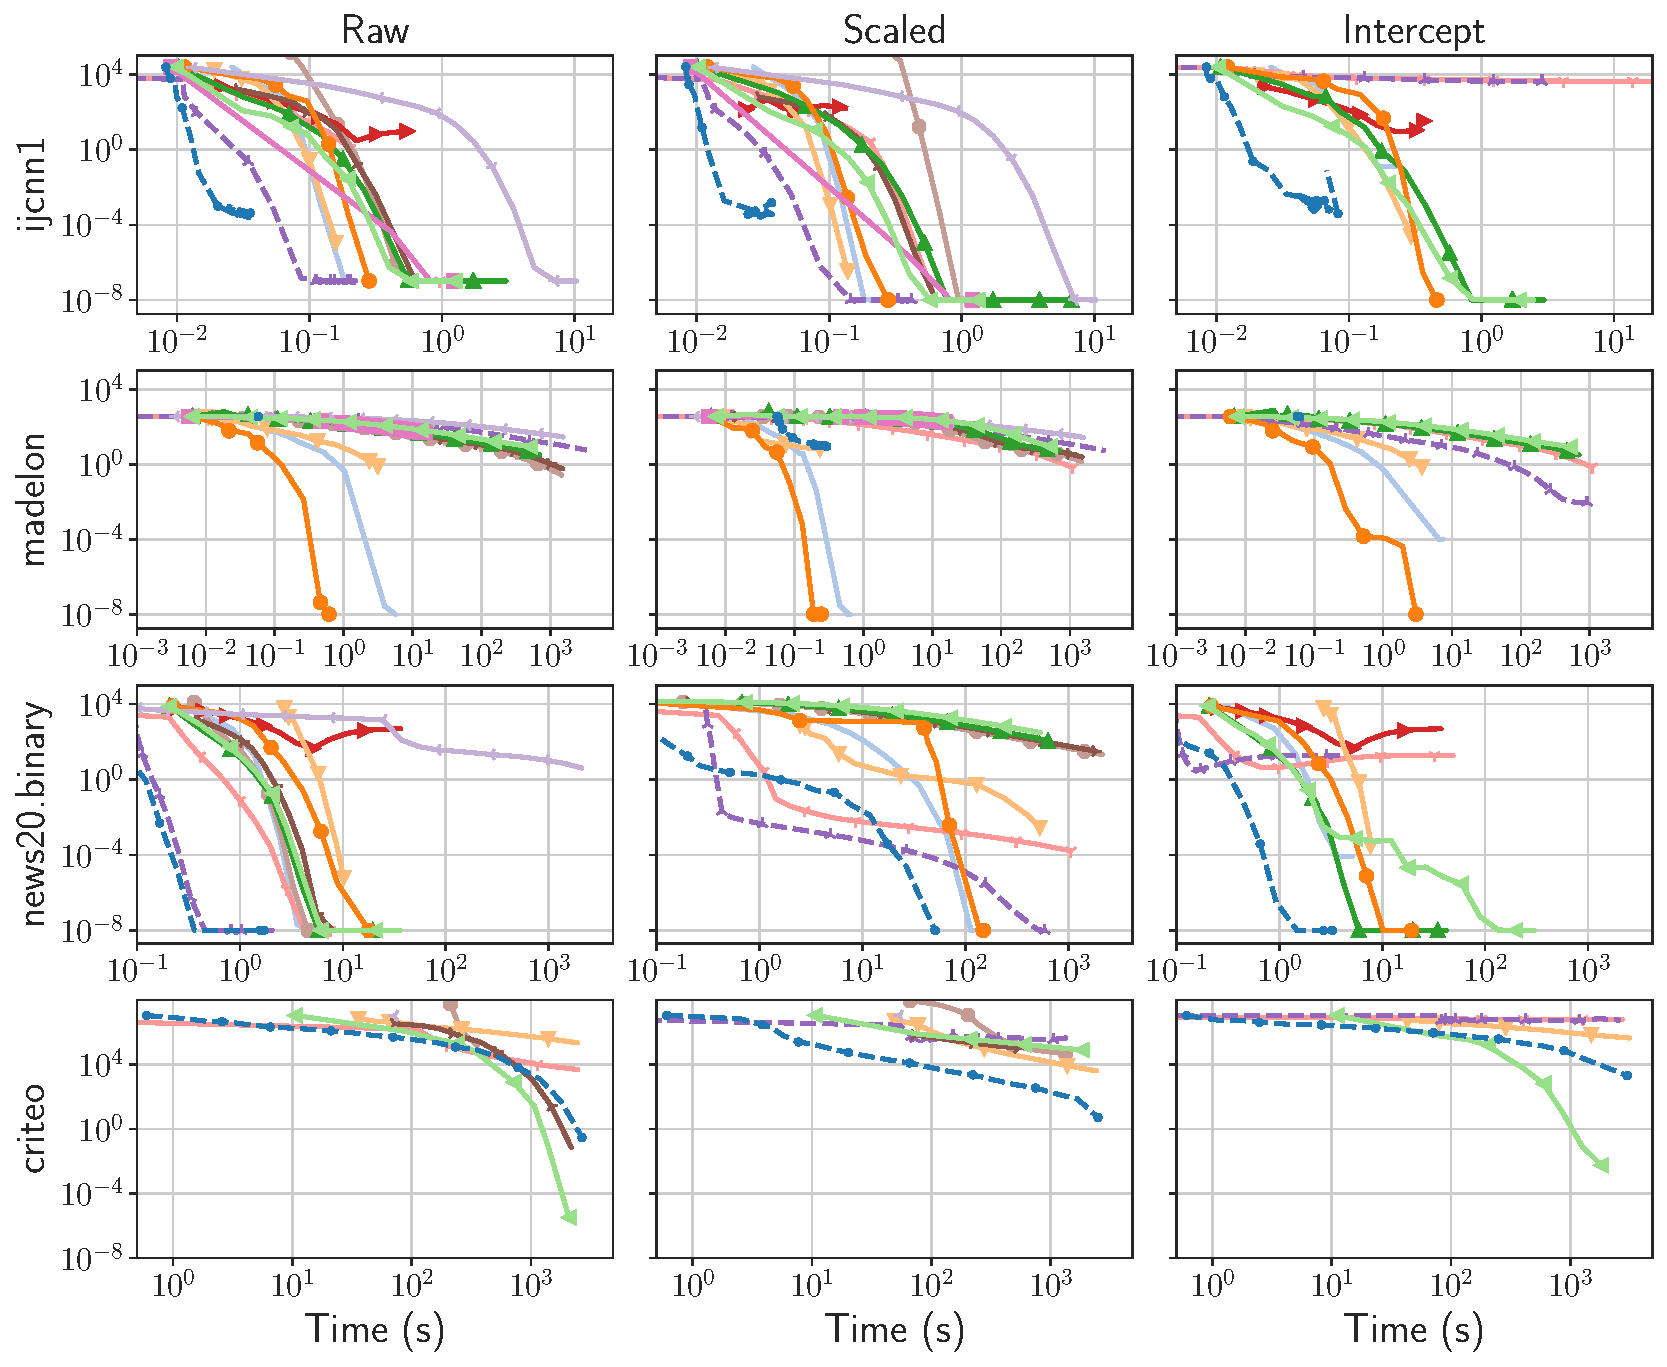
\includegraphics[width=\textwidth,trim={0 33em 0 0},clip]{logreg_l2_final.pdf}\\
% 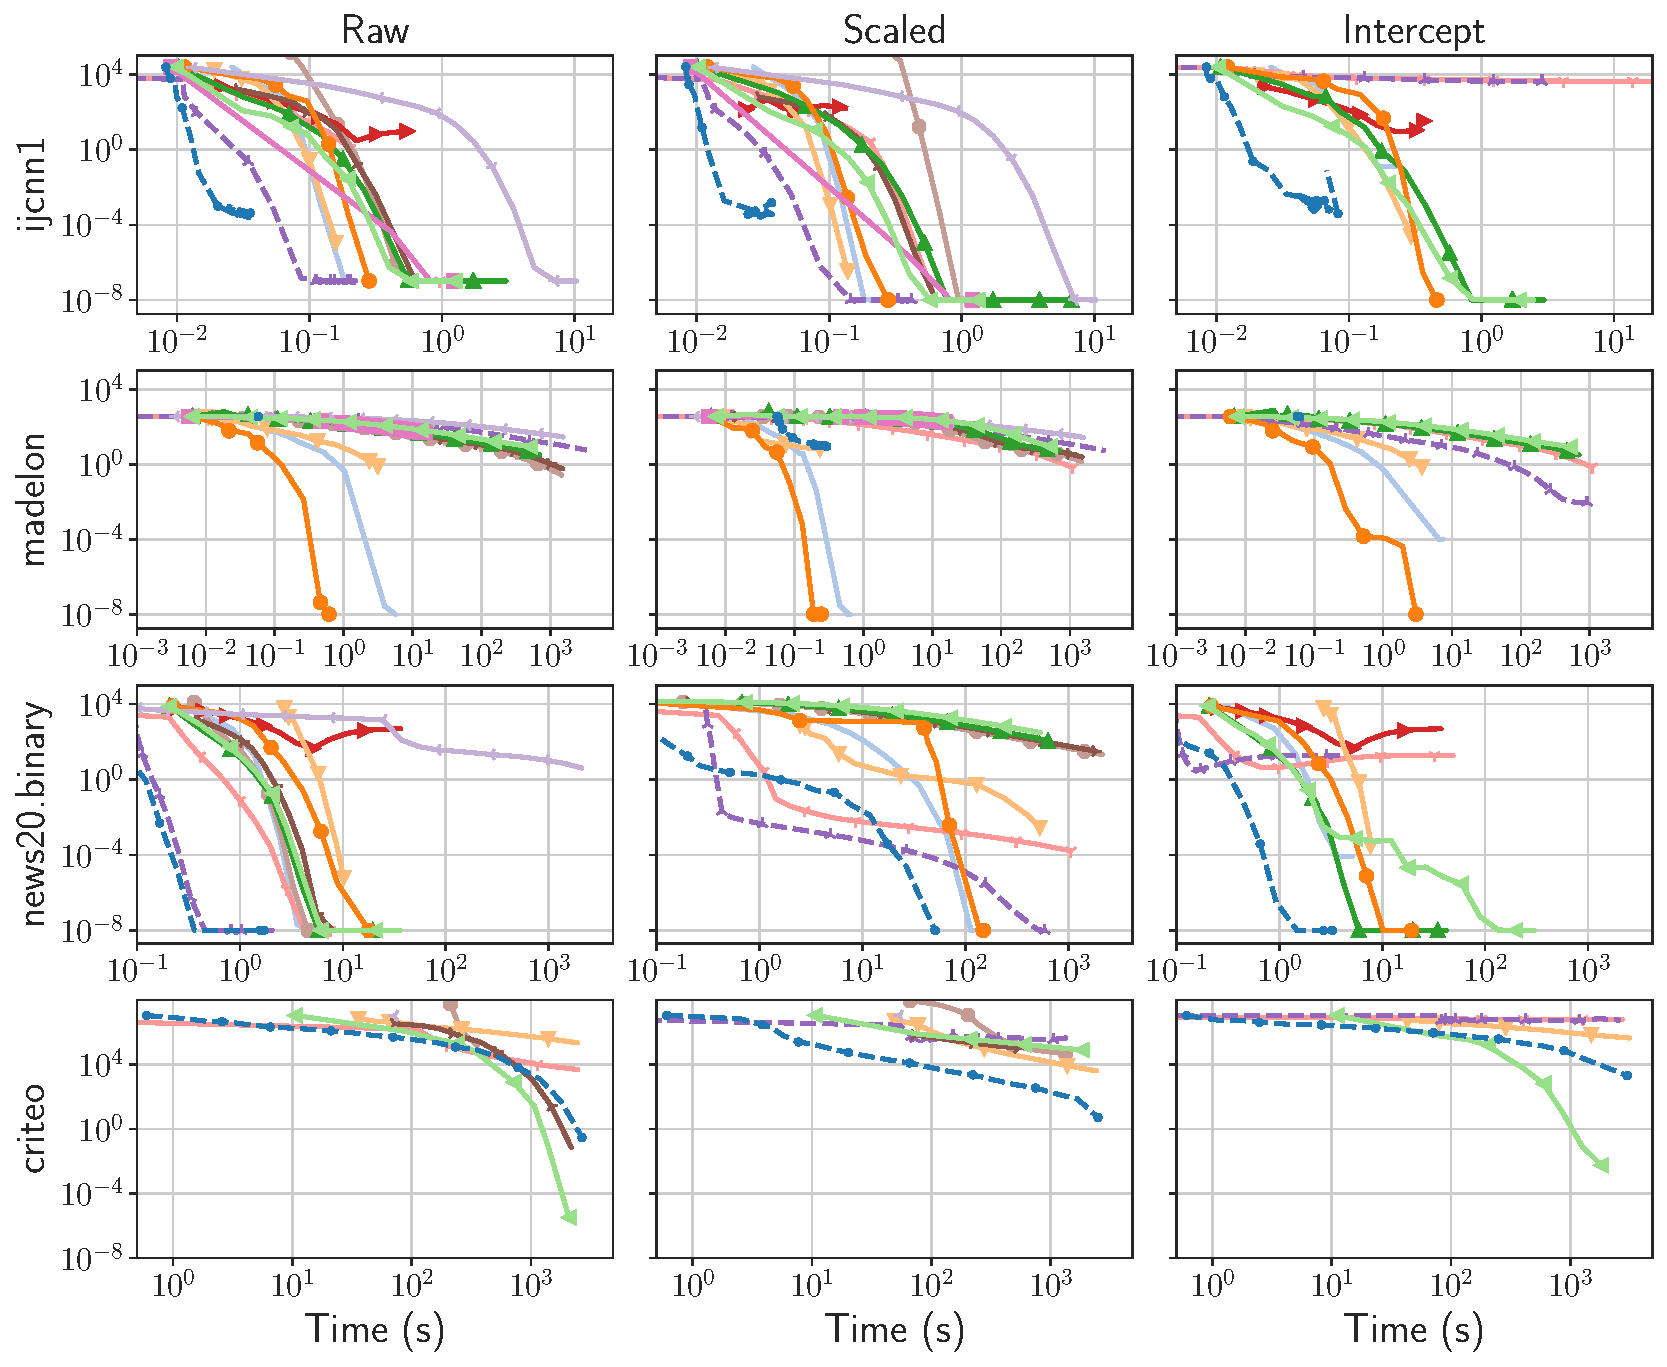
\includegraphics[width=\textwidth,trim={0 0 0 63em},clip]{logreg_l2_final.pdf}\\
% 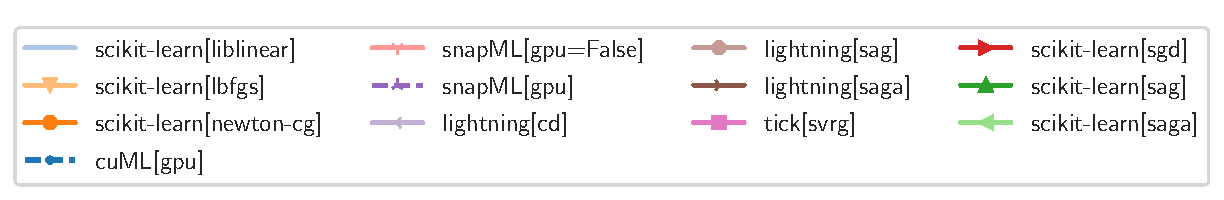
\includegraphics[width=\textwidth]{logreg_l2_final_legend}\\
% }

%%%%%%%%%%%%%%%%%%%%%%%%%%%%%%%%%%%%%%%%%%%%%%%%%%%%%%%%%%%%%%%%%%%%%%%%%%%%%%
% Benchmark logreg
%%%%%%%%%%%%%%%%%%%%%%%%%%%%%%%%%%%%%%%%%%%%%%%%%%%%%%%%%%%%%%%%%%%%%%%%%%%%%%
\headerbox{Some Other Benchmarks}{name=benchmarks,column=4,below=use-case-solver,span=2}{
%%%%%%%%%%%%%%%%%%%%%%%%%%%%%%%%%%%%%%%%%%%%%%%%%%%%%%%%%%%%%%%%%%%%%%%%%%%%%%
\vskip.1em
\begin{itemize}[itemsep=-2pt]
  \item Regularized Logistic Regression
  \item Total Variation Inverse Problems
  \item Quantile Regression
  \item Sparse Regression
  \item Non-Negative Least-squares
  \item Independent Component Analysis
\end{itemize}
\vspace{-7mm}
{\bf\centering\Large Add yours with our template!!\hskip3ex
\raisebox{-1em}{
\includegraphics[height=2.6em]{qr-template}}
\\}
}

%%%%%%%%%%%%%%%%%%%%%%%%%%%%%%%%%%%%%%%%%%%%%%%%%%%%%%%%%%%%%%%%%%%%%%%%%%%%%%
% Benchmark Lasso
%%%%%%%%%%%%%%%%%%%%%%%%%%%%%%%%%%%%%%%%%%%%%%%%%%%%%%%%%%%%%%%%%%%%%%%%%%%%%%
\headerbox{Lasso}{name=lasso,column=0,below=resnet,span=4}{
%%%%%%%%%%%%%%%%%%%%%%%%%%%%%%%%%%%%%%%%%%%%%%%%%%%%%%%%%%%%%%%%%%%%%%%%%%%%%%

% \[
%     \min_\beta\frac12\|y - X\beta\|_2^2 + \lambda\|\beta\|_1
% \]
\centering
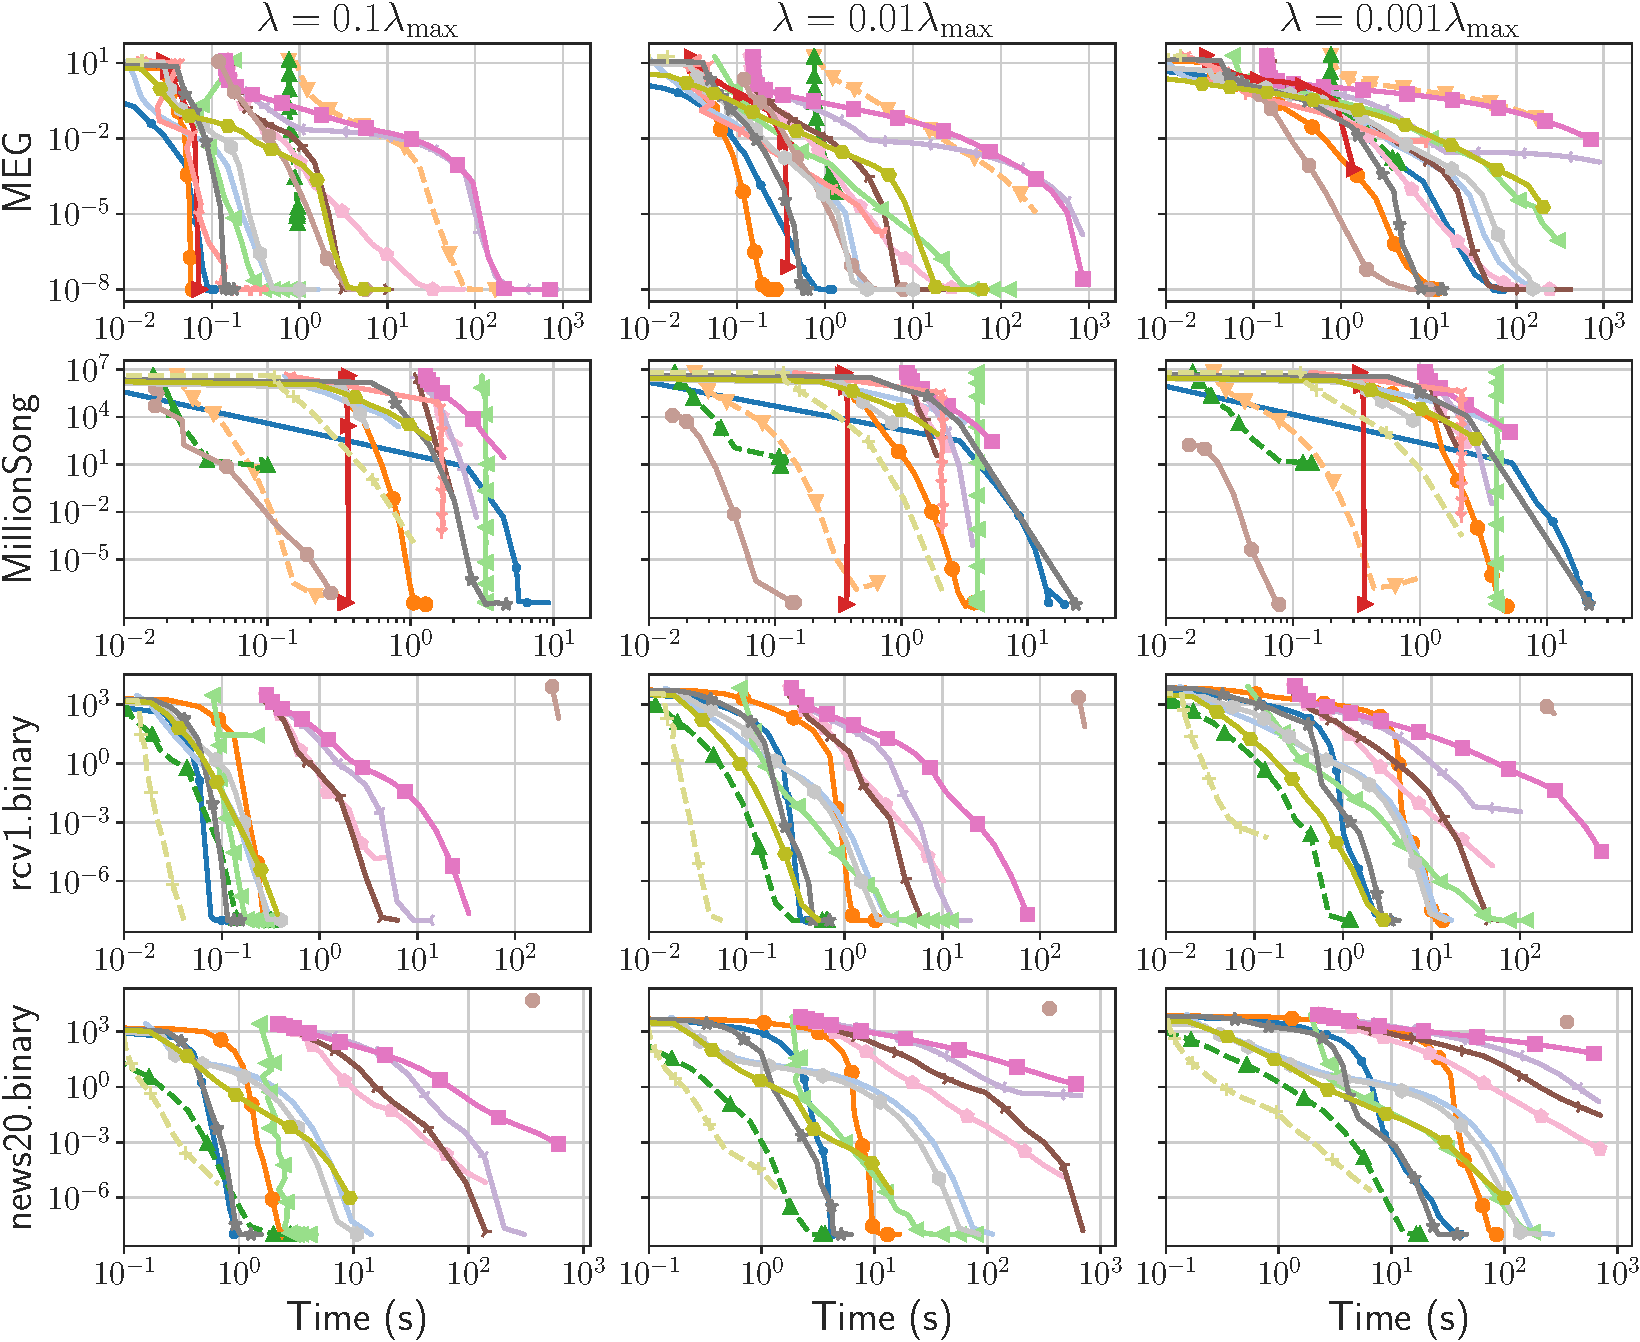
\includegraphics[width=0.9\textwidth,trim={0 48em 0 0},clip]{meg_rcv1_news20_MSD.pdf}\\
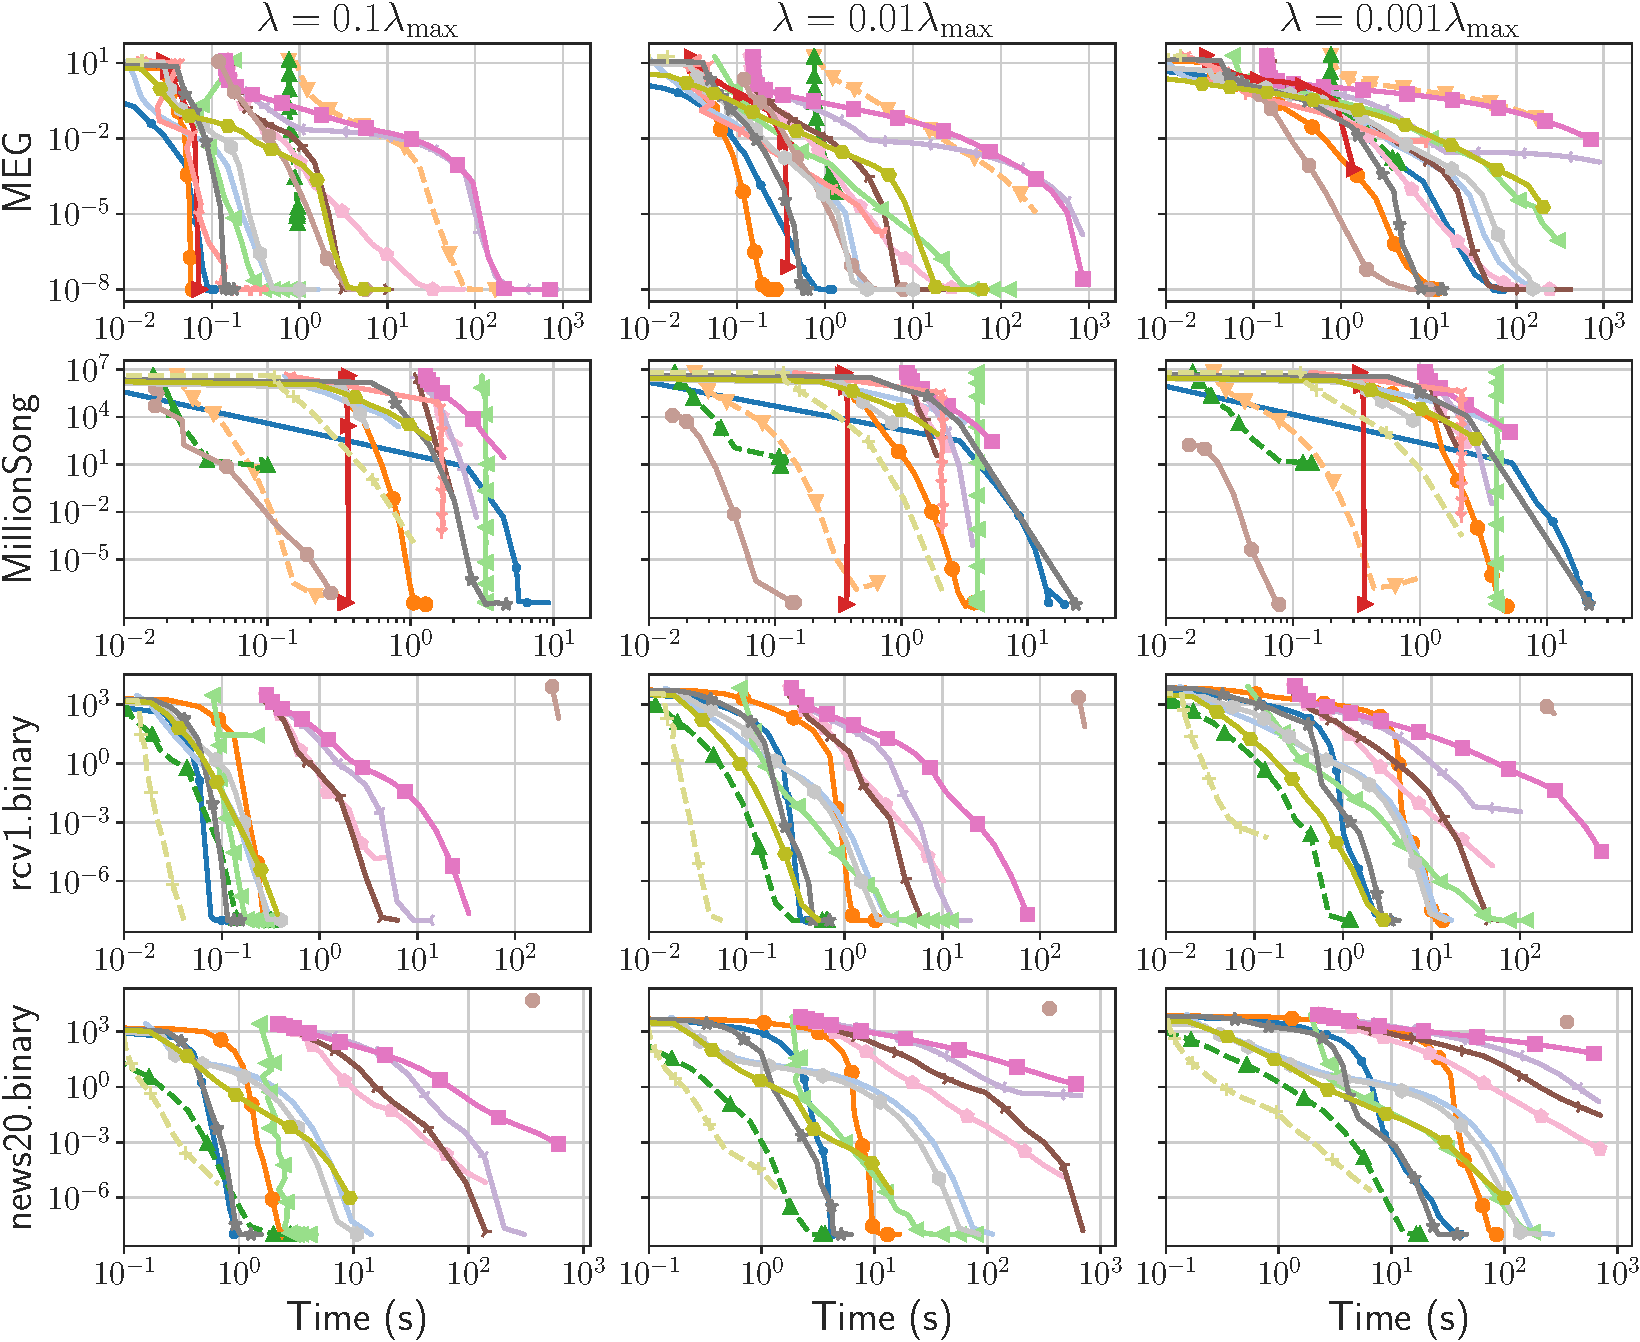
\includegraphics[width=\textwidth,trim={0 0 0 62em},clip]{meg_rcv1_news20_MSD.pdf}\\[.5em]
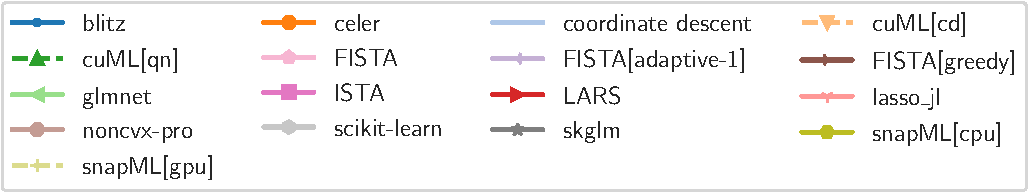
\includegraphics[width=.9\textwidth]{meg_rcv1_news20_MSD_legend}\\


}



\end{poster}

\end{document}

